
%(BEGIN_QUESTION)
% Copyright 2014, Tony R. Kuphaldt, released under the Creative Commons Attribution License (v 1.0)
% This means you may do almost anything with this work of mine, so long as you give me proper credit

Calculate the source voltage and current in this transformer circuit.  Assume an ideal transformer with no power losses at all:

$$\includegraphics[width=15.5cm]{i01080x01.eps}$$

$V_{source}$ = \hskip 80pt $I_{source}$ =

\vskip 10pt

\underbar{file i01080}
%(END_QUESTION)





%(BEGIN_ANSWER)

$V_{source}$ = 94.5 V \hskip 80pt $I_{source}$ = 42.0 mA

%(END_ANSWER)





%(BEGIN_NOTES)

{\bf This question is intended for exams only and not worksheets!}.

%(END_NOTES)


